\section{Introduction}
In this chapter the design method, seen on \cref{scenarioModel} is followed to create the interaction design for the program. The method focuses on the use of scenarios, which are about people performing activities in context by using technology, throughout the design process. In the model there are different design processes shown as clouds and the products of these processes shown as boxes. Each of the main processes Understanding, Envisionment, Evaluation and Design in designing interactive systems is used in the scenario based method. The following parts will discuss different products, their use in the model and the processes which they have been deducted from.

\begin{figure}[H]
	\centering
	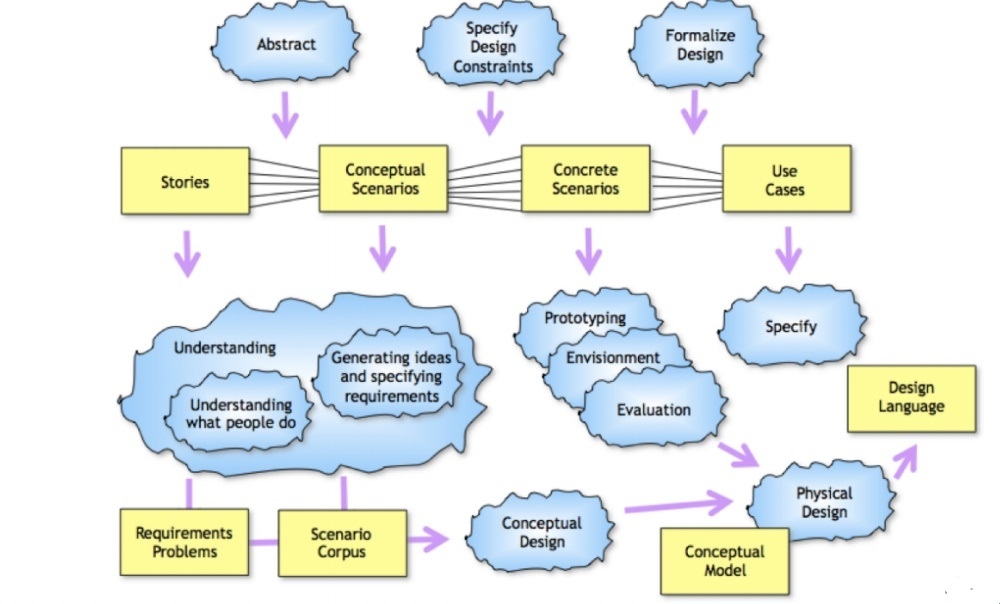
\includegraphics[width=1\textwidth]{Grafik/scenarioModel}
	\caption{Scenario-based design method}
	\label{scenarioModel}
\end{figure}